\documentclass[10pt,a4paper]{article}
\usepackage[slovak]{babel}
\usepackage[utf8]{inputenc}
\usepackage{amsmath}
\usepackage{amsfonts}
\usepackage{amssymb}
\usepackage[unicode]{hyperref}
\usepackage{graphicx}

\textwidth 6.5in
\oddsidemargin 0.0in
\evensidemargin 0.0in

\title{Poznámky z Úvodu do databázových systémov - materiál na štátnice}
\date{16.06.2012}
\author{Peter Csiba, petherz@gmail.com, \url{https://github.com/Petrzlen/fmfi-poznamky}} 

\begin{document}
\maketitle
\tableofcontents

\clearpage

%%%%%%%%%%%%%%%%%%%%%%%%%%%%%%%%%%%%%%%%%%%%%%%%%%%%%%%%%%%%%%%%%%%%%%%%%%%%%%%%
%%%%%%%%%%%%%%%%%%%%%%%%%%%%%%%%%%%%%%%%%%%%%%%%%%%%%%%%%%%%%%%%%%%%%%%%%%%%%%%%
\section*{Úvod}   

Text je poznámkami k oficiálnym \href{http://new.dcs.fmph.uniba.sk/index.php/Studium/Bakalarske/StatneSkusky}{štátnicovým otázkam} a boli spísané počas učenia sa na ne.
Poznámky sa nesnažia ísť do hĺbky (na to je H.Garcia-Molina, Ullman a Wikipédia).
Naopak, snažia sa priniesť intuitívnu predstavu o algoritmoch a pojmoch a dávať ich do súvisu.

Poznámky sú organizované podľa štátnicových otázok, snažia sa minimalizovať omáčku a nevysvetlujú a neuvádzajú do problematiky. Text je určený čitateľom, ktorý sa už s hlavnými pojmami stretli.
Autor považuje všetky otázky za rovnako dôležité a odporúča v prípade slabšieho pochopenia samostatne vypracovať niektoré staré \href{http://www.dcs.fmph.uniba.sk/~plachetk/TEACHING/DB2011/index.html}{písomky}.

Autor absolvoval základný test predmetu Úvodu do databázových systémov s hodnotením A, a má základné skúsenosti s administráciou a návrhom databáz. Napriek tomu autor \underline{neručí za kvalitu a úplnosť textu} a čitateľov \underline{aj} preto autor \underline{prudko odporúča pozrieť si aj iné zdroje}. Uvedieme citát\footnote{Dr. Tomas Plachetka, Uvod do databazovych systemov 2011/2012 Zima} ''Tieto slajdy sú sprievodcom pri prednáške, nie sú myslené ako náhrada
prednášky či nebodaj knihy. K príprave na skúšku nestačí len prečítať slajdy'', niečo také sú aj tieto poznámky.  

Nakoniec poznamenajme, že autor sa snažil písať pravdu a len pravdu, keďže jeho odpoveď na záverečných skúškach vychádza z tototo materiálu.
Ak čitateľ chce prispieť ku kvalite textu, nech autorovi napíše a ten mu udelí prístup do repozitára.

P.S. Autor zistil, že názvoslovie pijan, ľúbi, krčma, alkohol použil už napríklad \href{http://csip.sk/uploads/ullman.pdf}{Ullman}.

%%%%%%%%%%%%%%%%%%%%%%%%%%%%%%%%%%%%%%%%%%%%%%%%%%%%%%%%%%%%%%%%%%%%%%%%%%%%%%%%
%%%%%%%%%%%%%%%%%%%%%%%%%%%%%%%%%%%%%%%%%%%%%%%%%%%%%%%%%%%%%%%%%%%%%%%%%%%%%%%%
\section*{Úvod a motivácia databáz}
\paragraph{Účel.}
\begin{itemize}
\item Zobrazenie vybranej časti reality v počítačí.
\item Uchovávanie informácií v konzistentnom stave a ich pridávanie.
\item Poskytovanie informácií (dotazy, reporty - periodické správy). 
\item Ochrana informácií pred zničením a neoprávneným prístupom. 
\end{itemize}

\paragraph{Charakteristiky DBMS (Database Management System).}
\begin{itemize}
\item Dáta majú štruktúru, ktorá sa zriedka mení, objem dát je veľký.
\item Dáta nie sú uložené na užívateľovom počítači, pre prístup k dátam sa využíva počítačová sieť (klient-server).
\item Dotazy sú zložité.
\item Množstvo užívateľov pristupuje k dátam súčasne.
\item Vyžaduje sa vysoká priepustnosť.
\item Vyžaduje sa vysoká odolnosť voči poruchám.
\item Vyžaduje sa vysoký stupeň bezpečnosti.
\item Prístup koncových užívateľov k dátam musí byť jednoduchý(API, GUI).
\end{itemize}

\paragraph{Porovnanie dotazov v dátových modeloch.}
Vo všeobecnosti sa snažíme zbaviť všeobecných kvatifikátorov pomocou pravidla $\forall P \rightarrow \neg \exists \neg P$.

Máme tabuľky: 
\begin{itemize}
\item studenti(Student, Skupina)
\item rozvrh\_skupiny(Skupina, Miestnost, Cas)
\item rozvrh\_ucitelia(Ucitel, Skupina)
\end{itemize}

\begin{itemize}
\item \emph{Hovorovo.} Treba nájsť (všetky) štvorice [Student, Miestnost, Cas, Ucitel]
také, že ten učiteľ učí toho študenta v tej miestnosti a tom čase. 
\item \emph{Predikátový kalkul.}

\{[Student, Miestnost, Cas, Ucitel]: $\exists$ Skupina (Student, Skupina) $\wedge$ rozvrh\_skupiny(Skupina, Miestnost, Cas) $\wedge$ rozvrh\_ucitelia(Ucitel, Skupina)\}
\item \emph{Relačná algebra.}
$$
\Pi_{student, miestnost, cas, ucitel}(studenti \Join rozvrh_skupiny \Join rozvrh_ucitelia)
$$
\item \emph{Datalog (Prolog).}
\begin{verbatim}
rozvrh_studenti(Student, Miestnost, Cas, Ucitel) <--
\begin{verbatim}
  studenti(Student, Skupina),
  rozvrh_skupiny(Skupina, Miestnost, Cas),
  rozvrh_ucitelia(Učitel, Skupina).

? rozvrh_studenti(S, M, C, U)
\end{verbatim} 

\item \emph{SQL.}
\begin{verbatim}
SELECT S.student, RK.miestnost, RK.cas, RU.ucitel
FROM studenti S, rozvrh_skupiny RK, rozvrh_ucitelia RU
WHERE S.skupina=RK.skupina AND S.skupina=RU.skupina
\end{verbatim}

\end{itemize}

%%%%%%%%%%%%%%%%%%%%%%%%%%%%%%%%%%%%%%%%%%%%%%%%%%%%%%%%%%%%%%%%%%%%%%%%%%%%%%%%
%%%%%%%%%%%%%%%%%%%%%%%%%%%%%%%%%%%%%%%%%%%%%%%%%%%%%%%%%%%%%%%%%%%%%%%%%%%%%%%%
%TODO vynechava stranu, (asi) lebo article a section* a section
\section{Dátové modely} 
\href{http://en.wikipedia.org/wiki/Database_model}{Pozri Wikipédiu.}

\paragraph{Používané dátové modely.}
\begin{itemize}
\item Entitno-relačný. Pozri \ref{entity_relationship}. 
\item Relačný. Pozri \ref{relacny_kalkul} a \ref{relacna_algebra}. 
\item Navigačný (XML). Stromová štruktúra, dotazovací jazyk XPath a XQuery. 
\item Objektový. Niečo ako objekty v programovaní. Objekty okrem zapuzdrenia dát špecifikujú prístup k nim a k ich vzťahom, je možné s nimi programaticky narábať. Napríklad DOM (Document Object Model). 
\end{itemize}


%%%%%%%%%%%%%%%%%%%%%%%%%%%%%%%%%%%%%%%
\subsection{Trojschémová architektúra (ANSI sparc)}

\paragraph{Úrovne.}
\begin{itemize}
\item Konceptuálna úroveň (všeobecná databázová schéma). 
\item Interná úroveň (špecifikácia polí, kľúčov, indexov, ...).
\item Fyzická úroveň. Algoritmy a dátové štruktúry, využtie diskového priestoru. Pozri \ref{fyzicka_organizacia}.
\end{itemize}

\begin{center}
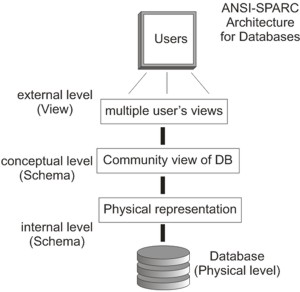
\includegraphics[scale=0.5]{db_ansi_sparc.jpg}
\end{center} 

\paragraph{Vlastnosti.}
\begin{itemize}
\item Nezávislý pohľad užívateľov. Každý môže použiť svoj dotazovací jazyk. 
\item Užívateľ nevidí fyzickú organizáciu dát. Tá sa môže zmeniť, bez toho, aby to užívateľ postrehol. 
\end{itemize}

%%%%%%%%%%%%%%%%%%%%%%%%%%%%%%%%%%%%%%%
\subsection{Entitno-relačný model}
\label{entity_relationship}

Máme entity (tabuľky, polia, ...) a vzťahy medzi nimi. 
\paragraph{Typy vzťahov.}
\begin{itemize}
\item One-to-one (1-1). Napríklad hlava a telo. 
\item One-to-many (1-n). Napríklad vozidlo a kolesá. 
\item Many-to-many (n-m). Napríklad kupujúci a produkt (táto dvojica nemusí byť unikátna).
\end{itemize}

\begin{center}
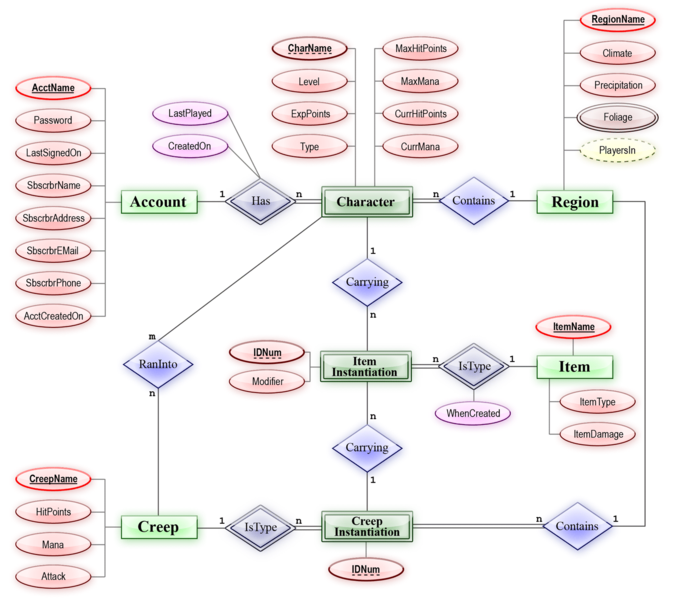
\includegraphics[scale=0.5]{db_entity_relationship.png}
\end{center} 

%%%%%%%%%%%%%%%%%%%%%%%%%%%%%%%%%%%%%%%
\subsection{Relačný model, relačná algebra}
Pozri \ref{relacny_kalkul} a \ref{relacna_algebra}. 

%%%%%%%%%%%%%%%%%%%%%%%%%%%%%%%%%%%%%%%
\subsection{Negácia a rekurzia v relačnej algebre}
Pozri \ref{relacna_algebra}. 

%%%%%%%%%%%%%%%%%%%%%%%%%%%%%%%%%%%%%%%
\subsection{Súvis relačnej algebry s inými dotazovacími jazykmi}
Pozri \ref{relacna_algebra_suvis}.
    
%%%%%%%%%%%%%%%%%%%%%%%%%%%%%%%%%%%%%%%%%%%%%%%%%%%%%%%%%%%%%%%%%%%%%%%%%%%%%%%%
%%%%%%%%%%%%%%%%%%%%%%%%%%%%%%%%%%%%%%%%%%%%%%%%%%%%%%%%%%%%%%%%%%%%%%%%%%%%%%%%
\section{Relačný kalkul} 
\label{relacny_kalkul}

Deklaruje výroky, ktoré ohraničujú výsledok dotazu. 
\paragraph{Použité pojmy.}
Je odporúčané vedieť matematickú logiku. 

\begin{itemize}
\item $n$-árna relácia (konečná, nekonečná). Usporiadané $n$-tice. Karteziánsky súčin. 
\item Atribúty - zložky $n$-tíc. Domény (typy atribútov) - množiny karteziánskeho súčinu. 
\item Predikát $P$ prislúchajúci relácií $R$- zobrazenie $R_P : R \mapsto$ \{true, false\}, pričom $R_P(A) = true \leftrightarrow A \in R$, kde $A$ je usporiadaná $n$-tica. V praxi medzi tým nerozlišujeme. 
\end{itemize}

\paragraph{Dotaz.}
Dotazy v relačnom kalkule sú logické formuly predikátovej logiky prvého rádu.
Formula by nemala mať voľné premenné. Výsledkom sú prvky relácie, ktoré spĺňajú formulu. 

%%%%%%%%%%%%%%%%%%%%%%%%%%%%%%%%%%%%%%%
\subsection{Predikátová interpretácia relačnej algebry}
??? Asi ide o prepis symbolov relačnej algebry do predikátovej logiky. 
%TODO 

%%%%%%%%%%%%%%%%%%%%%%%%%%%%%%%%%%%%%%%
\subsection{Negácia, doménovo nezávislé a bezpečné formuly}

\paragraph{Príklad dotazov.}
\begin{enumerate}
\item prvocisla1: $\{Z : (\forall X) (\forall Y) (krat(X,Y,Z) \rightarrow X = 1 \wedge Y = 1)\}$.
\item zlozene\_cisla: $\{Z : (\exists X) (\exists Y) (krat(X,Y,Z) \wedge X \neq 1 \wedge Y \neq 1)\}$.
\item prvocisla2: $\{Z : (\exists X) (\exists Y) (krat(X,Y,Z) \wedge Z \notin zlozene\_cisla) \}$.
\item prvocisla3: $\{Z : Z \notin zlozene\_cisla\}$.
\end{enumerate}
Tretiu formulu (reláciu, resp. množinu) sme získali dvojitou negáciou prvej a pravidlom $P \rightarrow Q \Leftrightarrow \neg P \vee Q$ (medzi krok je druhá formula). 

Formuly pre prvocisla1 a prvocisla3 sú \emph{nebezpečné}, keďže ich výsledom je napríklad aj ''petrzlen''.
V prvom prípade je implikácia pravdivá (lebo ľavá strana je nepravdivá) a v druhom prípade je to zjavné, keďže ''petrzlen'' nie je zložené číslo. 
Správna je len formula prvocisla2. 

\emph{Množina faktov} (nazývaná aj \emph{extenzionálna databáza (EDB)}) je \underline{konečná} množina, na ktorej je predikát v dotaze pravdivý (to zrejme neplati pre prvocisla1 a prvocisla3, ale platí pre prvocisla2 a zlozene\_cisla).
Neformálne, \emph{bezpečný dotaz} je taký, v ktorom sa každá premenná vyskytuje v aspoň jednom EDB v pozitívnom kontexte. Tj. chceme, aby sa premenná \underline{ne}vyskytovala v negovanej množine faktov (výroku). Napríklad v prvocisla3 je $Z$ v negatívnom kontexte.  

%%%%%%%%%%%%%%%%%%%%%%%%%%%%%%%%%%%%%%%
\subsection{Relačný kalkul (doménový)}

Myslím, že je to popísané v predošlých sekciách.
Pripomeňme, že \emph{domény} sú typy atribútov - množiny karteziánskeho súčinu.


%%%%%%%%%%%%%%%%%%%%%%%%%%%%%%%%%%%%%%%
\subsection{Súvis relačného kalkulu s inými dotazovacími jazykmi}
Základná intuícia. Celkom dobre sa doň prekladá z hovorového a jendoducho sa z neho konštruuje datalog, resp. relačná algebra.
V praxi nie je použiteľný, keďže ide o teoretický model (s potenciálne nekonečnými reláciami). 
    
%TODO 

%%%%%%%%%%%%%%%%%%%%%%%%%%%%%%%%%%%%%%%%%%%%%%%%%%%%%%%%%%%%%%%%%%%%%%%%%%%%%%%%
%%%%%%%%%%%%%%%%%%%%%%%%%%%%%%%%%%%%%%%%%%%%%%%%%%%%%%%%%%%%%%%%%%%%%%%%%%%%%%%%
\section{Datalog} 
\href{http://en.wikipedia.org/wiki/Datalog}{Datalog} je dotazovací jazyk s pravidlami určený pre deduktívne databázy, ktorý je syntakticky podmnožinou Prologu. Je založený na predikátovej logike prvého rádu (neumožňuje kvantifikovať množiny) a \underline{umožňuje rekurziu}. 

Odporúčame si pozrieť slide-i Plachetku pre ďalšie príklady dotazov.
Ideálne si niektoré úlohy treba vyskúšať v Datalógovom interpretery (tak sa to učí najlepšie).

%%%%%%%%%%%%%%%%%%%%%%%%%%%%%%%%%%%%%%%
\subsection{Syntax a sémantika Datalogových programov}

\paragraph{Syntax.}
Program pozostáva z množiny pravidiel - \emph{implikácií} - \emph{predikátov}, ktoré majú \emph{hlavu} a \emph{telo}\footnote{
Nie pätu. Poznámka autora. 
} (ľavá a pravá strana implikácie, resp. \emph{premisa} a \emph{dôsledok}). 
Napríklad:
\begin{verbatim}
1. krat(1, 1, 1) <-- TRUE.
2. krat(1, 1, 1).
3. zlozene_cislo(Z) <--
  krat(X, Y, Z),
  not X = 1,
  not Y = 1.
4. prvocislo(Z) <--
  krat(X, Y, Z),
  not zlozene_cislo(Z)
5. prvocislo(Z) <--
  krat(_, _, Z),
  not zlozene_cislo(Z)
\end{verbatim} 
Predikáty 1 a 2 a aj predikáty 4 a 5 sú sémanticky ekvivalentné. Premenné na ľavej strane sú kvantifikované $\forall$ a premenné na pravej strane $\exists$. Čiarka medzi atómami má význam AND. Bodka označuje koniec predikátu. \emph{Podcieľmi} nazývame atómy tela rozdelené čiarkami, napríklad 
  \verb|{krat(_, _, Z)}| a \verb|not zlozene_cislo(Z)| sú podcieľmi \verb|prvocislo(Z)|. 
V 5 používame \emph{anonymné premenné} ''\_''. Ich sémentika je rovnaká, ako keby sa použila ľubovoľná nepoužitá premenná. Poznmenajme, že v tele pravidla sú premenné implicitne kvantifikované $\exists$.
  
Alebo (disjunkcia) sa vyjadruje:
\begin{verbatim}
colour(F) <-- F = black
colour(F) <-- F = white
\end{verbatim} 
  
\paragraph{Ďalšie syntaktické pravidlá.}

\begin{itemize}
\item Argumentmi (hláv) predikátov môžu byť len jednoduché atribúty. Nemôžeme \verb|zlozene_cislo(f(f(Z,5)) <-- |. 
\item (Tvrdí Wiki, nie Plachetka). Každá premenná v hlave predikátu sa musí vyskytovať aj v nie negovanom podcieli predikátu (súvisí s bezpečnosťou). 
\end{itemize}

\paragraph{Sémantika.}
Je založená na relačnom kalkule (a matematickej logike). 
Niečo sa spomenulo vyššie, doplňujeme v ďalšej sekcií. 

\paragraph{Agregácia (subtotal).}
\begin{verbatim}
objednava_od_hp(K, V) <--
objednavky(K, V), dodava(hp, V, _, _).
answer(K, P) <--
subtotal(objednava_od_hp(K, V), [K], [P = count(V)]).
\end{verbatim} 

Príkaz \verb|subtotal| má tri parametre. Prvým je predikát, druhým je \emph{grupovací atribút} a tretím \emph{agregovací atribút}. Viac v \ref{rel_alg_agg}. 

Podobne sa dá definovať subtotal aj pre relačný kalkulus. 

%%%%%%%%%%%%%%%%%%%%%%%%%%%%%%%%%%%%%%%
\subsection{Súvis s relačným kalkulom}

Napríklad 
\begin{verbatim}
3. zlozene_cislo(Z) <--
  krat(X, Y, Z),
  not X = 1,
  not Y = 1.
\end{verbatim} 
je sémanticky ekvivalentným programom k $$
zlozene\_cisla: \{Z : (\exists X) (\exists Y) (krat(X,Y,Z) \wedge X \neq 1 \wedge Y \neq 1)\}.
$$


Existuje algoritmický predklad medzi týmito dvoma modelmi.
Algoritmus, ktorý prepisuje relačný kalkul do Datalogu pozostáva z nasledujúcich krokov (treba ich vedieť \underline{použiť}):

\begin{enumerate}
\item Premenovanie premenných, lokalizácia kvantifikátorov. Vlastne veta o variantoch z matematickej logiky. 

\item Eliminácia všeobecných kvantifikátorov a implikácií. Použijeme pravidlá $(\forall x)A(x) \leftrightarrow \neg (\exists x) \neg A(x)$ a $(A \rightarrow B) \leftrightarrow (\neg A \vee B)$.

\item Definícia pomocných predikátov. Chceme sa vyhnúť sekvencií $\neg (\exists X) povodny\_predikat(X)$. Definujeme preto pomocné predikáty: 
$$
\begin{array}{l}
\neg novy\_predikat \\
novy\_predikat \leftarrow (\exists X) povodny\_predikat(X).\\
\end{array} 
$$

\item Bezpečnosť pomocných predikátov. Pridáme k premenným ich dómeny:
$$
novy\_predikat \leftarrow domena(X) \wedge (\exists X) povodny\_predikat(X).
$$

\item Prepis do pravidiel Datalogu. Len zmeniť syntax:
\begin{verbatim}
answer <-- not novy_predikat.
novy_predikat <-- povodny_predikat(X).
\end{verbatim}

\end{enumerate}

Poznamenajme, že podobne existuje algoritmus, ktorý prepisuje datalogove dotazy do SQL (tiež treba vedieť použiť). 

%%%%%%%%%%%%%%%%%%%%%%%%%%%%%%%%%%%%%%%
\subsection{Výpočet dotazu na Datalogový program}

Datalog počíta \emph{minimálny model} programu (minimálne relácie, pre ktoré je daný program splnený). Inými slovami, Datalog vracia najmenšiu množinu, pre ktorú sú splnené všetky potrebné predikáty, na ktorých závisí dôsledok (dotaz). Tj. neuvažuje také výsledky, pre ktoré sú predpoklady nesplnené. Napríklad program: 
\begin{verbatim}
colour(black).
colour(white).
? colour(C).
\end{verbatim}
by mohol vrátiť aj ''mrkva'', lebo nič tomu neodporuje.

Minimálny model existuje pre každý \emph{bezpečný program} (ktorý sa definuje prakticky rovnako, ako v relačnom kalkule).

%%%%%%%%%%%%%%%%%%%%%%%%%%%%%%%%%%%%%%%
\subsection{Negácia}

\paragraph{Russelov paradox.}
\begin{verbatim}
man(barber).
man(mayor).
shaves(barber, X) <-- man(X), not shaves(X, X).
? shaves(barber, barber)
\end{verbatim}

Paradox nenastáva, keďže pravidlo je definované ako implikácia. Výsledok nemôže byť FALSE,
lebo by predpoklad bol splnený. Ak je výsledok TRUE, tak \verb|man(X), not shaves(X, X) --> shaves(barber, X)| platí. 

%%%%%%%%%%%%%%%%%%%%%%%%%%%%%%%%%%%%%%%
\subsection{Bezpečnosť Datalogových programov}

\emph{Bezpečný predikát} je taký, ktorého všetky premenné vyskytytujúce sa v hlave, sú viazané v EDB. 

\emph{Bezpečný program} má všetky svoje predikáty bezpečené. 

(Zopakujeme) Minimálny model existuje pre každý bezpečný program (ktorý sa definuje prakticky rovnako, ako v relačnom kalkule).
 
Všeobecne platí, že anonymné premenné v negovaných EDB podcieľoch
nespôsobujú problém s bezpečnosťou.
 
Pán Šturc definujeme slabšie podmienky. 
    
%%%%%%%%%%%%%%%%%%%%%%%%%%%%%%%%%%%%%%%%%%%%%%%%%%%%%%%%%%%%%%%%%%%%%%%%%%%%%%%%
%%%%%%%%%%%%%%%%%%%%%%%%%%%%%%%%%%%%%%%%%%%%%%%%%%%%%%%%%%%%%%%%%%%%%%%%%%%%%%%%
\section{Relačná algebra} 
\label{relacna_algebra}

Hovorí AKO sa má niečo vypočítať. Operuje len nad konečnými množinami (aby neboli problémy s negáciami). Formalizuje SQL. Viac na \href{http://en.wikipedia.org/wiki/Relational_algebra}{Wikipédií} - náhodny poznatok odtiaľ: Reflexívno tranzitívny uzáver sa nedá relačnou algebrou vyjadriť. 
 
V tejto sekcií budeme implicitne veľkými písmenami značiť $m$-tice atribútov nad $n$-reláciami $r$ ako $X = (X_1, X_2, \ldots, X_m)$ (nemusí $n=m$). 

%%%%%%%%%%%%%%%%%%%%%%%%%%%%%%%%%%%%%%%
\subsection{Operátory relačnej algebry}

\paragraph{Operátory.}
\begin{itemize}
\item Projekcia $\Pi$. Nech $r$ má atribúty $Y$, potom $\Pi_X(r)$ vznikne kopírovaním riadkov $r$, pričom sa skopírujú len tie atribúty, ktoré sú v $X$. Treba eliminovať potenciálne duplicity. 
\item Selekcia $\Sigma$. Nech $c$ je podmienka a $X$ atribúty $r$, potom $\Sigma_{c(X)} = \{X:r(X) \wedge c(X)\}$. 
\item Kartézsky súčin $\times$. Relácie $r_1$ a $r_2$, atribúty $X$, $Y$ pričom $X \cap Y = \emptyset$, potom $r_1 \times r_2 = \{[X,Y]:r_1(X) \wedge r_2(Y)\}$.
\item Join (theta-join). Podmienka $c$, relácie $r_1$ a $r_2$, atribúty $X$, $Y$ pričom $X \cap Y = \emptyset$, potom $r_1 \Join_{c(X,Y)} r_2 = \{[X,Y]:r_1(X) \wedge r_2(X) \wedge c(X,Y)\}$.
\item Premenovanie $P_{r_2(Y)}(r1)$ atribútov relácie.
\item Natural join $\Join$. Nech $r_1$ je typu\footnote{Všetky atribúty $r_1$ je zjednotenie $X$ a $Z$} $r_1(X, Z)$ a $r_2$ je typu $r_2(Y, Z)$, pričom $Z$ sú spoločné
atribúty $r_1$ a $r_2$. Potom $r_1 \Join r_2 = \{[X,Y,Z]:r_1(X,Z) \wedge r_2(Y,Z)\}$, pričom
spoločné atribúty (atribúty s rovnakým menom) sú testované na
rovnosť a sú kopírované iba raz. Natural join sa dá vyjadriť projekciou a theta-joinom. 
\item Tradičné množinové $\Cap, \Cup, \ldots $ .
\item Eliminácia duplikátov $r_2 = \Delta(r_1)$.
\end{itemize}

\paragraph{Optimalizácia výpočtu.}
Použitie operátorov sa zvykne zapisovať v strome, kde operátory sú vrcholy a argumenty (relácie) hrany.
Pre jeden výraz môže existovať viacero výpočtovo ekvivalentných stromov.
Zopár pravidiel na konštrukciu optimálneho: 
\begin{itemize}
\item Selekciu urob čo najskôr.
\item Vyhýbaj sa kartézskym súčinom, nahraď ich joinom. Ak
nasleduje selekcia, pridaj ju do joinovacej podmienky.
\item Postupnosť unárnych operácií (selekcie a projekcie) spoj do
jednej operácie a zviaž s nasledujúcou operáciou.
\item Výsledok opakovaného podvýrazu ulož, ak je veľkosť tabuľky
malá, tak ju materializuj. 
\item Nájdi optimálne poradie joinov technikou dynamického
programovania. Poradí pre N tabuliek je zhruba $2^N$ (binárne stromy). 
\end{itemize}

%%%%%%%%%%%%%%%%%%%%%%%%%%%%%%%%%%%%%%%
\subsection{Multimnožinová interpretácia relácií}

Plachetka: "Relačná algebra počíta nad multimnožinami". Na Wikipédií som to nenašiel explicitne spomenuté a takisto sme operátory definovali pre množiny. V každom prípade je možné jednoduchým spôsobom rozšíriť definície na \emph{multimnožiny}\footnote{Rovnaký prvok sa môže vyskytnúť viackrát}. Kto nevie, \href{http://en.wikipedia.org/wiki/Multiset}{Wikipédia}. 

Niektoré základné vlastnosti operácií sa nezachovávajú, ako napríklad $S \cup S = S$. 

%%%%%%%%%%%%%%%%%%%%%%%%%%%%%%%%%%%%%%%
\subsection{Grupovanie a agregácia}
\label{rel_alg_agg}
(Skopírovaný slide.)

O každom atribúte $x \in X$ platí buď 
\begin{itemize}
\item $x$ je atribútom $r_1$ (v tom prípade atribútu $X$ hovoríme
        \emph{grupovací atribút}), alebo
\item $x = AGG(Y)$, kde $Y$ je atribútom $r_1$ a $AGG$ je nejaká
     agregačná funkcia, ktorá zo stĺpca Y vyrába jednu hodnotu (v
         tom prípade atribútu x hovoríme \emph{agregovaný atribút})
V SQL je $AGG \in \{SUM, COUNT, AVG, STDEV, MAX, MIN\}$.
\end{itemize}

Operátor $\Gamma_X(r_1)$
\begin{enumerate}
\item najprv vyrobí z relácie $r_1$ skupiny, pričom riadky v každej zo
skupín majú rovnaké hodnoty grupovacích atribútov
\item potom vypočíta agregované atribúty pre každú skupinu.
\end{enumerate}
Výsledkom je tabuľka, v ktorej každej skupine prináleží jeden
riadok.
 
Implementuje sa projekciou (multimnožinovou) a vyhodením duplikátov. 

SQL:
\begin{tabular}{lc}
SELECT $<S\_attr>$ & 5 \\
FROM $r_1$, $r_2$, ..., $r_n$ & 1 \\
WHERE $<w\_cond>$ & 2 \\
GROUP BY $<G\_attr>$ & 3 \\
HAVING $<h\_cond>$ & 4 \\
\end{tabular}

Relačná algebra: 
$$\Pi_{S_attr}(\Sigma_{h_cond}(\Gamma_{G_attr, agg(Attr)}(\Sigma_{w_cond}(r_1 \times r_2 \times \ldots \times r_n))))$$.


%%%%%%%%%%%%%%%%%%%%%%%%%%%%%%%%%%%%%%%
\subsection{Rekurzia, výpočet pevného bodu}

Podľa Wiki základná relačná algebra nevie rekurziu (to je celkom zrejmé). 
Plachetkov slide: 

Operátor \emph{minimal fixpoint} (tranzitívny uzáver) $\Phi(<vyraz>)$ iteruje výraz, kým sa relácie použité vo výraze
menia (t.j. kým sa mení obsah aspoň 1 relácie výrazu)

Príklad:
\begin{tabular}{ll}
ancestor &:= parent(X, A) \\
ancestor &:= ancestor $\cup \Pi_{X,A}$(ancestor $\Join$ parent) \\
ancestor &:= ancestor $\cup \Pi_{X,A}$(ancestor $\Join$ parent) \\
... & \\
\end{tabular}
sa zapíše ako\\
ancestor := $\Phi$($\cup \Pi_{X,A}$(ancestor $\Join$ parent)) \\

Výpočet pevného bodu patrí do predmetu Základy teórie programovania (blok B1). 
Naivný algortimus: \\
\verb|answer = {};| \\
\verb|do| \\
\verb|{| \\
\verb|answer = iteration_step(|$\Phi_1$\verb|);| \\
\verb|answer = iteration_step(|$\Phi_2$\verb|);| \\
\verb|...| \\
\verb|answer = iteration_step(|$\Phi_n$\verb|);| \\
\verb|} while answer changed; /* anywhere inside this loop */| \\

Oveľa viac v \href{http://www.dcs.fmph.uniba.sk/~plachetk/TEACHING/DB2011/db2011_5.pdf}{slide-och z roku 2011}.

%TODO str.197-220 

%%%%%%%%%%%%%%%%%%%%%%%%%%%%%%%%%%%%%%%
\subsection{Súvis relačnej algebry s inými dotazovacími jazykmi}
\label{relacna_algebra_suvis}

SQL bolo inšpirované relačnou algebrou. 
    
%%%%%%%%%%%%%%%%%%%%%%%%%%%%%%%%%%%%%%%%%%%%%%%%%%%%%%%%%%%%%%%%%%%%%%%%%%%%%%%%
%%%%%%%%%%%%%%%%%%%%%%%%%%%%%%%%%%%%%%%%%%%%%%%%%%%%%%%%%%%%%%%%%%%%%%%%%%%%%%%%
\section{Jazyk SQL (Structured Query Language)} 
\emph{SQL} je jazykom pre prístup k relačným databázou navrhnutým na základe relačnej algebry a relačného kalkulu. 
Predpokladáme, že väčšina pozná (alebo si aspoň myslí, že pozná). Takže len stručne. 
Kto nevie, tak \href{http://en.wikipedia.org/wiki/SQL}{Wikipedia}. 

%%%%%%%%%%%%%%%%%%%%%%%%%%%%%%%%%%%%%%%
\subsection{Programovanie v SQL (DDL, DML)}

SQL je typový jazyk.

Poznamenajme, že SQL používa trojhodnotovú logiku: \{TRUE, FALSE, NULL\}
a tabuľky nie sú množinami, ale zoznammi (rovnaká $n$-tica - riadok - sa môže vyskytovať viackrát). Obe sú v spore s relačnou algebrou. 

Ďalej poznamenajme, že tabuľka nemusí byť materializovaná, môže byť dočasná alebo trvalá. 

\paragraph{DDL (Data Definition Language).}
Vytvára (mení, maže) štruktúru dát, relácie, indexy, užívateľov (a prístupové práva), triggery, ... . 

DDL a DML sú podmnožinami jazyka SQL. 

\begin{itemize}
\item CREATE. Najčastejšie CREATE TABLE.
\item ALTER. 
\item RENAME.
\item DROP. Navždy vymazať. 
\item TRUNCATE. Vyprázdniť. 
\end{itemize}

\paragraph{DML (Data Manipulation Language).}
Slúži na prístup, pridávanie, zmenu a zmazanie dát. 

\begin{itemize}
\item SELECT. 
\item INSERT. 
\item UPDATE.
\item DELETE. Navždy vymazať. 
\item MERGE. Vyprázdniť. 
\end{itemize}

\paragraph{Kľúčové slová pre SELECT.}
\begin{itemize}
\item FROM. Z tabuľky.  
\item WHERE. Kde podmienka. 
\item \verb|[FULL, LEFT, RIGHT] [INNER, OUTER] JOIN|. Spájanie viacerých tabuliek podľa podmienky. Odporúčame si pozrieť \href{http://www.codinghorror.com/blog/2007/10/a-visual-explanation-of-sql-joins.html}{grafické vysvetlenie}. Najbežnejší je LEFT INNER JOIN (resp. len JOIN). [FULL, LEFT, RIGHT] hovorí, z pohľadu ktorej JOINujeme a OUTER (default je INNER) hovorí, že zahŕňame aj riadok, ktorý nemá pár. 
\item CROSS. Kartézsky súčin. 
\item UNION. Množinové zjednotenie dvoch tabuliek. UNION ALL je spojenie.
\item INTERSECT. Množinový prienik dvoch tabuliek. 
\item DISTINCT. Množinové správanie.    
\item EXISTS. Či SELECT vracia prázdny výsledok. 
\item ANY. Ľubovoľný vyhovujúci prvok z tabuľky. Použitie sa dá obísť, ide skôr o skratku. 
\item LIMIT. Obmedzenie počtu výstupných riadkov.
\item ORDER BY. Usporiadanie výstupu.
\end{itemize}

\paragraph{Agregácia.}
\begin{itemize}
\item GROUP BY. Agregácia.  
\item COUNT.
\item SUM.
\item AVG. 
\end{itemize}

\paragraph{NULL.}
Poznamenajme, že hodnota NULL sa môže chovať kontraintuitívne. 
Napríklad: 
\begin{verbatim}
SELECT r.C
FROM r
WHERE A < 1 OR A >= 1
\end{verbatim} 
nevráti riadky, kde $A=0$. 

\paragraph{Index.}
Uľahčujú vyhľadávanie, väčšinou sú implementované binárnymi vyhľadávacími stromami.
Tj. namiesto vyhľadávania v čase $O(n)$ máme $O(logn)$.

%%%%%%%%%%%%%%%%%%%%%%%%%%%%%%%%%%%%%%%
\subsection{Negácia a rekurzia v SQL}

O negácií to isté ako o negácií v Datalogu. 

Rekurzia v SQL je možná, napr. pomocou WITH, ktorý definuje dočasnú tabuľku. Rekurzia nastáva, keď sa odvolávame na tabuľku, ktorú práve definujeme. Koho viac zaujíma, môže si pozrieť \href{http://sqlanywhere.blogspot.sk/2012/04/example-recursive-union.html}{praktický príklad}. 

Konstra rekurzívneho programu pre UNION ALL: 
\begin{verbatim}
01. <typical_recursive_union> ::= WITH RECURSIVE <local_view_name>
02. "(" <alias_name_list> ")"
03. AS "(" <initial_query_specification>
04. UNION ALL
05. <recursive_query_specification> ")"
06. <outer_query_specification>
07. [ <order_by_clause> ]
08. [ <for_clause> ]
\end{verbatim} 

%%%%%%%%%%%%%%%%%%%%%%%%%%%%%%%%%%%%%%%
\subsection{Súvis SQL s inými dotazovacími jazykmi}

Bol postavený na relačnej algebre (pozri \ref{relacna_algebra}) a relačnom kalkule \ref{relacny_kalkul}. Existujú priamočiare algortimické transformácie s Datalogom a relačnou algebrou (operátorový strom). 
 
\paragraph{Konverzia z Datalogu.}
Existuje jednoduchý algortimus na preklad Datalogu do SQL,
využíva konštrukcie na vytváranie dočasných tabuliek: 
\begin{verbatim}
WITH r AS (SELECT ...),
SELECT ...
\end{verbatim} 
alebo
\begin{verbatim}
CREATE TEMPORARY TABLE r AS (SELECT ...);
SELECT ...
\end{verbatim}
alebo permanentnú, možno nie materializovanú: 
\begin{verbatim}
CREATE VIEW r AS (SELECT ...);
SELECT ...
\end{verbatim}

Hlavne CREATE VIEW si odporúčame pozrieť. 

%%%%%%%%%%%%%%%%%%%%%%%%%%%%%%%%%%%%%%%%%%%%%%%%%%%%%%%%%%%%%%%%%%%%%%%%%%%%%%%%
%%%%%%%%%%%%%%%%%%%%%%%%%%%%%%%%%%%%%%%%%%%%%%%%%%%%%%%%%%%%%%%%%%%%%%%%%%%%%%%%
\section{Teória navrhovania relačných báz dát} 

V tejto sekcií predpokladáme, že všetky spomínané datábázy sú relačné. 

\paragraph{Niektoré používané techniky.}
\begin{itemize}
\item \href{http://en.wikipedia.org/wiki/Structured_analysis}{SAD} (Structured Analysis and Design). Zachytáva procesy aj dáta naraz. Technika z roku 1980.
\begin{center}
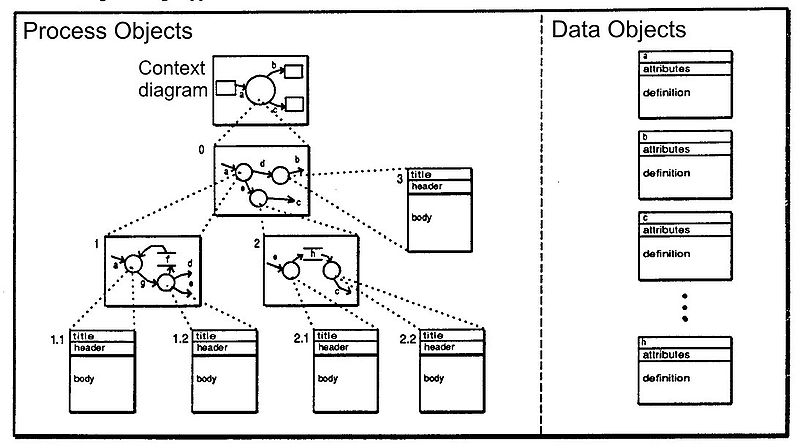
\includegraphics[scale=0.5]{db_sad.jpg}
\end{center}
\item DFD (Data-Flow Diagrams). Znnázorňuje, ako dáta prúdia cez systém, vstupy, výstupy. 
\begin{center}
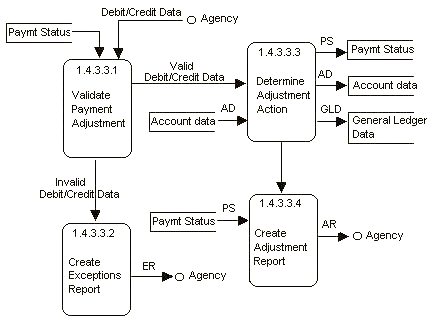
\includegraphics[scale=0.5]{db_dfd.png}
\end{center}
\item UML (Unified Modeling Language).S tým sa musel stretnúť každý, napríklad pri Design Patternoch. 
\begin{center}
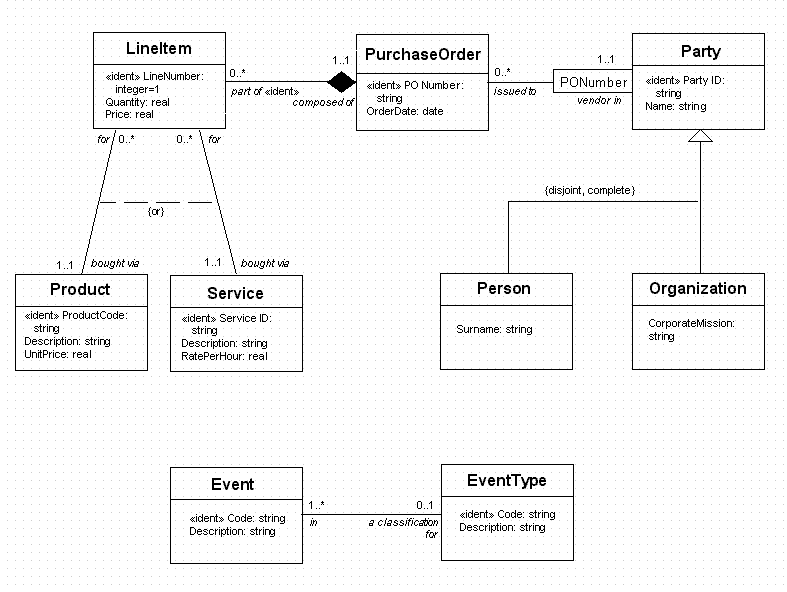
\includegraphics[scale=0.5]{db_uml.png}
\end{center}
\item ER (Enitity Relationship). S tými sme sa už stretli, sú najvhodnejšie pre relačné databázy (ako už názov napovedá). Nevýhodou je, že nezachytávajú ako sa entity menia. 
\begin{center}
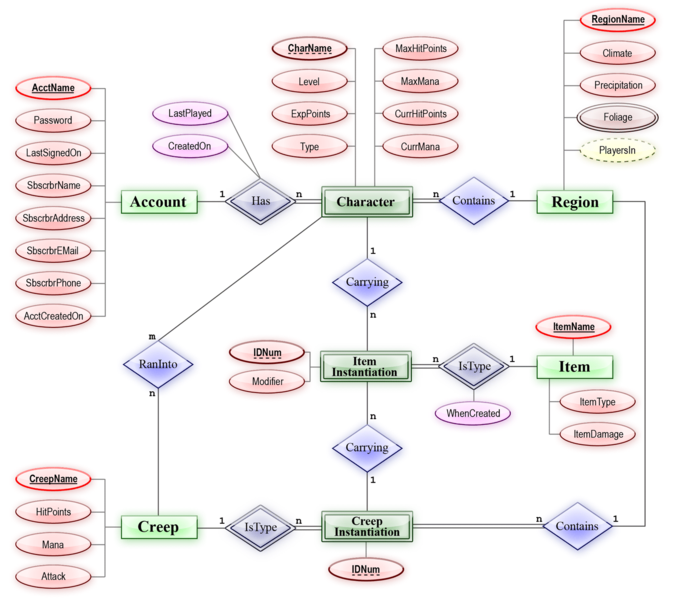
\includegraphics[scale=0.5]{db_entity_relationship.png}
\end{center}
\end{itemize}

Existujú softwareové nástroje, ktoré výrazne uľahčujú ich tvorbu, resp. vedia konvertovať textovú schému na takéto diagramy (je ich dosť). 

\paragraph{Kroky návrhu.}
\begin{itemize}
\item \emph{Koncepčný návrh}. Vytvorí sa diagram pre databázu a jej relácie. Zaujímajú nás entity a už menej ich atribúty a vôbec ich typy. 
\item \emph{Logický návrh}. Typy atribútov, bezpečnostný model, optimalizácia (normalizácia, ...), kľúče. Predklad do SQL (ako normu pre relačné DB) môžeme považovať za takýto krok. Treba vedieť syntax \verb|CREATE TABLE| a \href{http://dev.mysql.com/doc/refman/5.5/en/innodb-foreign-key-constraints.html}{hlavne} \verb|FOREIGN KEY (id) REFERENCES (table)| a ktomu prislúchajúci \verb|ON DELETE [CASCADE, SET NULL, RESTRICT=NO ACTION]|, ktoré hovoria čo sa má spraviť, keď sa vymaže FOREIGN KEY. 
\item \emph{Fyzický návrh}. Mapovanie návrhu na konkrétny DBMS (DB Management System). 
\end{itemize}

Výsledkom sú vytvorené tabuľky, kľúče, indexy, constrainty, užívateľské kontá,
procedúry vkladania/vynechávania dát, pohľady (VIEWs), prístupové práva atď.

\paragraph{Pravidlá dobrého návrhu.}
\begin{itemize}
\item \emph{Vyhýbať sa redundancií}. Ak sa dá niečo vypočítať, tak si to nepamätáme (jedine kvôli optimalizácií). Hlavným dôvodom je potenciálna nekonzistentnosť dát.  
\item \emph{Vyhýbať sa slabým entity setom}. To sú také, ktoré nevedia odpovedať na všetky (zmysluplné) otázky. Štandardne \emph{fan trap} - zlé poradie vzťahov entít v reťazi  a \emph{chasm trap} - chýbajúca závislosť (v trojici).
\item \emph{Nepoužívať entity set, ktorý sa dá nahradiť atribútom}. 
\end{itemize}

Prudko odporúčame pozrieť si \href{http://www.dcs.fmph.uniba.sk/~plachetk/TEACHING/DB2011/db2011_6.pdf}{slide-i Plachetku} pre názorné grafické ukážky chýb. 

%%%%%%%%%%%%%%%%%%%%%%%%%%%%%%%%%%%%%%%
\subsection{Funkčné závislosti}

\paragraph{Úvod a označenia.}
Chceme odstrániť redundanciu a znej plynúcu potenciálnu nekonzistentnosť. 

Ďalej budeme $X_i$ označovať \emph{inštanciu} množiny atribútov $X$ relácie $r$. 
Inštanciou rozumieme riadok (prvok relácie) s projekciou na $X$.
Ďalej, predikátom $r(X_i,Y_j, \ldots, Z_k)$ označujeme pre inštancie $(X_i,Y_j, \ldots, Z_k)$, či existuje spojená inštancia $(X_i,Y_j, \ldots, Z_k)$ v $r$.
Spojenou inštanciou\footnote{Definovali sme si len pre dočasné potreby, nevieme, či sa používa aj v odbornej literatúre.} 
rozumieme inštanciu $S$, ktorá má všetky atribúty relácie $r$. V prípade, že pre nejaké $X \cap Y \neq \emptyset$, tak inštancie $X_i$ a $Y_j$ musia mať na atribútoch $X \cap Y$ rovnaké hodnoty.  
Teraz sme vysvetľovali niečo, čo je takmer zrejmé, formalizmom, ktorý môže na prvé čitanie zmiasť. 

\paragraph{Definícia.}
\emph{Funkčná závislosť} $X \rightarrow Y$ práve vtedy keď 
$$(\forall X_1)(\forall Y_1,Y_2)(\forall Z_1) (r(X_1, Y_1, Z_1) \wedge r(X_1, Y_2, Z_1) \Rightarrow (Y_1 = Y_2)).$$

Odteraz ''$\Rightarrow$'' implikácia a ''$\rightarrow$'' funkčná závislosť.
Definujme makro $XY \equiv X \cup Y$. 

%%%%%%%%%%%%%%%%%%%%
\paragraph{Armstrongove axiómy.} 
\begin{itemize}
\item Reflexívnosť. $X \supseteq Y \Rightarrow X \rightarrow Y$.
\item Rozšírenie (augmentation). $(\forall Z)(X \rightarrow Y \Rightarrow (XZ \rightarrow YZ))$.
\item Tranzitívnosť. $(X \rightarrow Y \wedge Y \rightarrow Z) \Rightarrow (X \rightarrow Z)$.
\end{itemize}
 
Mali by ste vedieť dokázať (potom to ale nie sú axiómy, ale teorémy). 
 
Armstrongové axiómy sú úplne: 
Funkčná závislosť $X \rightarrow Y$ sa dá odvodiť z $F$ pomocou
Armstrongovych axióm práve vtedy, keď $X \rightarrow Y$ je logickým
dôsledkom\footnote{Učiteľ Matematickej logiky by sa nad týmto výrokom pozastavil. Logický dôsledok chápeme asi ako intuitívny pojem.} $F$.

 
%%%%%%%%%%%%%%%%%%%%
\paragraph{Niektoré ďalšie vlastnosti.}
 
\begin{itemize}
\item Union rule. $(X \rightarrow Y \wedge X \rightarrow Z) \Rightarrow (X \rightarrow YZ)$.
\item Pseudotranzivita. $(X \rightarrow Y \wedge WY \rightarrow Z) \Rightarrow (WX \rightarrow WZ)$.
\end{itemize}

Mali by ste vedieť dokázať z Armstrongových.
Všimneme si, že keď $r$ nemá funkčné závislosti, tak $r$ nemá redundantné dáta.  

%%%%%%%%%%%%%%%%%%%%
\paragraph{Uzáver množiny atribútov.}
(Skopírovaný slide.)

Nech $X$ je množina atribútov a $F$ množina funkčných
závislostí. Potom \emph{uzáverom množiny atribútov} $X$ vzhľadom na $F$
rozumieme množinu $X^+$ všetkých atribútov $Y$ takých, že $X \rightarrow Y$ je
(logickým) dôsledkom funkčných závislostí $F$. 
 
\begin{verbatim}
X+ : = X;
repeat
for each U --> V in F do
if U in X+ then X+ := X+ union V;
while niečo sa pridalo do X+;
\end{verbatim}

Optimalizácia: každá závislosť sa použije práve raz, po použití ju
možno vynechať. (Teda uzáver sa počíta v lineárnom čase\footnote{
Na $F$ sme použili všetky Armstrongove axiómy (urobili sme niečo ako reflexívno tranzitívny uzáver). 
}.)

%%%%%%%%%%%%%%%%%%%%
\paragraph{Uzáver množiny funkčných závislostí.}
(Skopírovaný slide.)

Označme $F^+$ množinu všetkých funkčných závislostí,
ktoré sú dôsledkom funkčných závislostí z $F$ (t.j. ktoré sa dajú
odvodiť z $F$ použitím Armstrongovych axióm). Množinu $F^+$ budeme
nazývať \emph{uzáverom množiny funkčných závislostí} $F$.

Je dosť rozsiahla, chceme uvažovať len vhodnú podmnožinu. 
\emph{Maximálna funkčná závislosť} - nemôže vynechať atribút z ľavej strany ani pridať atribút k pravej strane tak, aby sme neporušili jej platnosť. 

%%%%%%%%%%%%%%%%%%%%%%%%%%%%%%%%%%%%%%%
\subsection{Pokrytie a minimálne pokrytie množiny funkčných závislostí}
Množina funkčných závislostí $G$ \emph{pokrýva} množinu funkčných závislostí $F$ práve vtedy keď $G^+ \supseteq F^+$. 
Stačí testovať, či vieme odvodiť každú funkčnú závislosť z F pomocou G (polynomiálne).     

\emph{Kanonická funkčná závislosť} - je maximálna a na pravej strane má práve jeden atribút.     

\emph{Minimálne pokrytie množiny funkčných závislostí} - je pokrytie pozostávajúce len z kanonických funkčných závislostí. 

\paragraph{Polynomiálny algoritmus na výpočet minimálneho pokrytia.}
\begin{enumerate}
\item Nahraď $X \rightarrow Y$ množinou \{$X \rightarrow A$, $A \in Y$, $A$ je jednoduchý (jednotkový) atribút\}
\item Vynechaj všetky redundantné (odvoditeľné) atribúty na ľavých stranách
$X \rightarrow A$ (každý atribút treba testovať práve raz). 
\item Vynechaj všetky redundantné (odvoditeľné z ostatných) závislosti $X \rightarrow A$ (opakuj tento
krok s redukovanou množinou funkčných závislostí, kým
žiadna závislosť nie je redundantná, každú závislosť treba
testovať práve raz). Viac v slide-och. 

\end{enumerate}

%%%%%%%%%%%%%%%%%%%%%%%%%%%%%%%%%%%%%%%
\subsection{Nadkľúče a kľúče}

\emph{Kľúč} je (neformálne) minimálna množina atribútov, ktorá
jednoznačne identifikuje entitu. Kľúčov môže byť viac. \emph{Primárny
kľúč} je niektorý z kľúčov a označuje sa počiarknutím atribútov,
ktoré ho tvoria. Primátny kľúč by mal byť minimálny možný, odporúča sa použiť zástupcu \emph{surrogate key} (napr. AUTO INCREMENT v SQL). 

Formálne je \emph{nadkľúč} množina atribútov $K$ taká, že $K \rightarrow U$, kde $U$ sú všetky atribúty relácie $r$. \emph{Kľúčom} nazývame \underline{minimálny} (v zmysle množinovej inklúzie) nadkľúč $r$ (môže ich teda byť viacej).

Algoritmus na nájdenie kľúčov existuje len exponenciálny (určite ste ho vedeli na teste). Plachetka odporúča úplne preberanie kľúčov zhora (najdlhších), po najkratšie. Výpočet sa reprezentuje binárnym stromom, kde sa v každom vrchole množina aitribútov vetví podľa toho, či  daný atribút zahrnieme, alebo nezahrnieme do potenciálneho kľúča (a podčiarkujeme si pritom atribúty, ktoré určite chceme zahrnúť). 

%%%%%%%%%%%%%%%%%%%%%%%%%%%%%%%%%%%%%%%%%%%%%%%%%%%%%%%%%%%%%%%%%%%%%%%%%%%%%%%%
%%%%%%%%%%%%%%%%%%%%%%%%%%%%%%%%%%%%%%%%%%%%%%%%%%%%%%%%%%%%%%%%%%%%%%%%%%%%%%%%
\section{Normálne formy} 

Tabuľky, ktoré nie sú v normálnych formách, môžu napríklad viesť k stratám závislosti pri vymazávaní alebo nekonzistentným dátam pri zmenách (viac v \href{http://www.dcs.fmph.uniba.sk/~plachetk/TEACHING/DB2011/db2011_8.pdf}{slide-och}).

\paragraph{Relačná schéma.}
\emph{Relačná schéma} je množina atribútov $U$ a množina funkčných závislostí $F$, ktoré platia v relácií $r$. Tj, rozdeľujeme tabuľky na viacero tabuliek. 

\emph{Dekompozícia relačnej schémy} sú relácie $r_i$ a funkčné závislosti $F_i$, pričom $r_i$ vznikli projekciou $r$ (a vymazaním duplikátov), $\Cup_i r_i = U$ a $F^+ \supseteq F_i$ (nepridali sa nové závislosti).

\emph{Bezstratová dekompozícia} práve vtedy, keď $r = \Pi_{r_1}(r) \Join \cdots Join \Pi_{r_n}(r)$. Všetky funkčné závislosti sa museli zachovať, inak by sa relácia $r$ neobnovila. Poznamenajme, že $r_i$ sme definovali ako relácie a v $\Pi_{r_1}(r) $ ich používame ako množiny atribútov. 

\paragraph{Prvá normálna forma (1NF).} (Historický problém) Atribúty definujeme nad doménami s atomickými hodnotami (nie napr. \verb|enum|). V skutočnosti sa definuje trocha \href{http://en.wikipedia.org/wiki/First_normal_form}{inak} - pridávajú sa množinové vlastnosti riadkov a stĺpcov. 

\paragraph{Druhá normálna forma (2NF).} (Historický problém) Žiadny atribút v $r_i$ nezávisí iba na časti kľúča $r_i$ a každá z $r_i$ je v 1NF. Tj., ak je kľúč (=minimálny nadkľúč) v tvare $ABC$, tak v tabuľke neexistujú funkčné závislosti, ktorých ľavé strany sú $A,B,C,AB,BC$ alebo $AC$. 

\begin{center}
\begin{tabular}{l|l|l}
$Employee$ & $Skill$ & $Current Work Location$ \\
\hline
Jones &	Typing &	114 Main Street \\
Jones &	Shorthand &	114 Main Street \\
Jones &	Whittling &	114 Main Street \\
Bravo &	Light Cleaning &	73 Industrial Way \\
Ellis &	Alchemy &	73 Industrial Way \\
Ellis &	Flying &	73 Industrial Way \\
Harrison &	Light Cleaning &	73 Industrial Way \\
\end{tabular}
\end{center}

Jediným kľúčom tabuľky je $(Employee, Skill)$, ale tabuľka nie je v 2NF, lebo existuje funkčná závislosť $Employee \rightarrow Current Work Location$.

%%%%%%%%%%%%%%%%%%%%%%%%%%%%%%%%%%%%%%%
\subsection{3NF, BCNF}

\paragraph{Tretia normálna forma (3NF).} (Plachetka) Relačná schéma $(r,F)$ je v 3NF práve vtedy, keď je v 2NF a pre každú (platnú) funkčnú závislosť $X \rightarrow Y$ platí, že buď $X$ je nadkľúč v $r$, alebo $Y$ je časťou nejakého kľúča v $r$. 
(\href{http://en.wikipedia.org/wiki/Third_normal_form}{Wikipédia}, silnejšia podmienka) Relačná schéma $(r,F)$ je v 3NF práve vtedy, keď je v 2NF a pre každú (platnú) pre každý atribút $U_i$ platí, že sa buď vyskytuje v šavej strane nejakého kľúča $r$, alebo je odvoditeľný z každého nadkľúča $r$.

Testovanie 3NF je NP ťažké, ale jej konštrukcia je polynomiálna. 

Ak to správne chápem, tak pri dekompozícií na $r_i$ musí podmienka 3NF platiť pre každú $r_i$ a nie pre celú $r$ (intuícia hovorí, že pri uvažovaní celej $r$ by to bola blbosť). 
Plachetka na ďalších slide-och potvrdzuje. 

\paragraph{Boyce-Coddova normálna forma (BCNF).} (Plachetka) Je v 2NF a pre každú platnú funkčnú závislosť $X \rightarrow Y$ platí, že $X$ je nadkľúč (\href{http://en.wikipedia.org/wiki/Boyce\%E2\%80\%93Codd_normal_form}{Wikipédia dodáva}, že $\neg (X \supseteq Y)$. 

Platí, že BCNF je prísnejšie ako 3NF (a zvykne sa preto označovať aj 3.5NF). 
Konštrukcia bezstratovej dekompozície do BCNF je NP ťažké, takisto, ako overenie jej existencie. 

\paragraph{Príklad 3NF a nie BCNF.}
Ak máme reláciu $ABC$ a funkčné závislosti $AB \rightarrow C$ a $C \rightarrow B$,
tak je v 3NF ($AB$ je kľúč) ale nie v BCNF, lebo $C$ nie je kľúč v $r$. Rozloženie na $(AC)$ a $(BC)$ (podľa naivného algoritmu) pomôže (bezstratovosť: $AC$ je kľúč). 

%%%%%%%%%%%%%%%%%%%%%%%%%%%%%%%%%%%%%%%
\subsection{Algoritmy pre dekompozíciu do normálnych foriem}

\paragraph{Naivný 3NF.} Nájdi nevyhovujúcu funkčnú závislosť (exponenciálne), minimalizuj ju na $X \rightarrow Y$ a rozlož príslušnú reláciu na relácie $r-Y$ a $XY$. 

\paragraph{Polynomiálny 3NF.} Nájdi minimálne pokrytie funkčnými závislosťami (polynomiálne). Pre každú $X \rightarrow Y$ z nich vytvor reláciu $XY$. Ak táto dekompozícia je stratová, pridaj reláciu pre ľubovoľný kľúč (bezstratovosť je ekvivalentná s existenciou takej tabuľky).

\paragraph{Naivný BCNF.} Nájdi nevyhovujúcu funkčnú závislosť (exponenciálne), minimalizuj ju na $X \rightarrow Y$ a rozlož príslušnú reláciu na relácie $r-Y$ a $XY$. 

%%%%%%%%%%%%%%%%%%%%%%%%%%%%%%%%%%%%%%%
\subsection{Bezstratovosť dekompozície}
(Názor autora, nesúhlasí s algoritmom v slide-och). 

\paragraph{Algoritmus.}
Relačná schéma $(r,F)$ s atribútmi $U_1,\ldots,U_n$ a s dekompozíciou $(r_1, F_1),\ldots,(r_m, F_m)$.

\begin{tabular}{ll}
1. & Vytvor maticu $S[i,j] = 1$ ak $U_j \in r_i$, inak $S[i,j] = 0$.\\
2. & Zvyšok opakuj, kým sa niečo mení:\\
3. & Pre každý $(X \rightarrow Y) \in F$:\\
4. & Ak pre riadok $r_i$, platí $(\forall U_j \in X)S[i,j]=1$, tak nastav $(\forall U_j)S[i,j]=1$.\\
\end{tabular}

Ak ľubovoľný riadok pozostáva zo samých jednotiek, tak je bezstratová. Všimnime si, že riadky sú medzi sebou nezávislé a reprezentujú atribúty, ktoré sa dajú odvodiť z atribútov relácií $r_i$. 
Inak povedané, dekompozícia je bezstratová, ak existuje relácia, z ktorej atrbútov sa dá odvodiť funkčnými závislosťami ostatné atribúty v $U$. 

\paragraph{Diskusia.}
    
%%%%%%%%%%%%%%%%%%%%%%%%%%%%%%%%%%%%%%%%%%%%%%%%%%%%%%%%%%%%%%%%%%%%%%%%%%%%%%%%
%%%%%%%%%%%%%%%%%%%%%%%%%%%%%%%%%%%%%%%%%%%%%%%%%%%%%%%%%%%%%%%%%%%%%%%%%%%%%%%%
\section{Transakcie} 
%%%%%%%%%%%%%%%%%%%%%%%%%%%%%%%%%%%%%%%
\subsection{Požiadavky na transakčný systém (ACID)}
%%%%%%%%%%%%%%%%%%%%%%%%%%%%%%%%%%%%%%%
\subsection{Architektúra transakčného systému}
%%%%%%%%%%%%%%%%%%%%%%%%%%%%%%%%%%%%%%%
\subsection{Rozvrhy}
%%%%%%%%%%%%%%%%%%%%%%%%%%%%%%%%%%%%%%%
\subsection{Triedy sériovateľnosti a obnoviteľnosti}
    
%%%%%%%%%%%%%%%%%%%%%%%%%%%%%%%%%%%%%%%%%%%%%%%%%%%%%%%%%%%%%%%%%%%%%%%%%%%%%%%%
%%%%%%%%%%%%%%%%%%%%%%%%%%%%%%%%%%%%%%%%%%%%%%%%%%%%%%%%%%%%%%%%%%%%%%%%%%%%%%%%
\section{Implementácia sériovateľnosti a obnoviteľnosti v transakčných systémoch} 
%%%%%%%%%%%%%%%%%%%%%%%%%%%%%%%%%%%%%%%
\subsection{Testy sériovateľnosti}
%%%%%%%%%%%%%%%%%%%%%%%%%%%%%%%%%%%%%%%
\subsection{Algoritmy izolácie, zámky, časové pečiatky, validácia}
%%%%%%%%%%%%%%%%%%%%%%%%%%%%%%%%%%%%%%%
\subsection{Uviaznutie (deadlock) a metódy riešenia uviaznutia}
%%%%%%%%%%%%%%%%%%%%%%%%%%%%%%%%%%%%%%%
\subsection{Algoritmy obnovy, log-file, checkpointing, backup}
    
%%%%%%%%%%%%%%%%%%%%%%%%%%%%%%%%%%%%%%%%%%%%%%%%%%%%%%%%%%%%%%%%%%%%%%%%%%%%%%%%
%%%%%%%%%%%%%%%%%%%%%%%%%%%%%%%%%%%%%%%%%%%%%%%%%%%%%%%%%%%%%%%%%%%%%%%%%%%%%%%%
\section{Fyzická organizácia} 
\label{fyzicka_organizacia}

%%%%%%%%%%%%%%%%%%%%%%%%%%%%%%%%%%%%%%%
\subsection{Dvojúrovňový model pamäti a organizácie dát}
%%%%%%%%%%%%%%%%%%%%%%%%%%%%%%%%%%%%%%%
\subsection{Indexové stromy, hashovanie}
%%%%%%%%%%%%%%%%%%%%%%%%%%%%%%%%%%%%%%%
\subsection{Operátory fyzickej algebry}
%%%%%%%%%%%%%%%%%%%%%%%%%%%%%%%%%%%%%%%
\subsection{Implementácia vybraných fyzických operátorov (merge-sort, nested-loop join)}


%%%%%%%%%%%%%%%%%%%%%%%%%%%%%%%%%%%%%%%%%%%%%%%%%%%%%%%%%%%%%%%%%%%%%%%%%%%%%%%%
%%%%%%%%%%%%%%%%%%%%%%%%%%%%%%%%%%%%%%%%%%%%%%%%%%%%%%%%%%%%%%%%%%%%%%%%%%%%%%%%
\clearpage
\section*{Referencie a odporúčaná literatúra}
\begin{itemize}                                
\item \href{http://www.dcs.fmph.uniba.sk/~plachetk/TEACHING/DB2011/index.html}{Úvodu do databázových systémov - Plachetka}.        
\item \href{http://www.dcs.fmph.uniba.sk/~sturc/databazy/uvod/}{Úvodu do databázových systémov - Šturc} - v niečom detailnejší.        
\item \href{http://infolab.stanford.edu/~widom/cs145/}{Úvodu do databázových systémov - Stanford University} - základ podobný.


\item \href{http://csip.sk/uploads/plachetka\_uvod\_do\_databaz\_2011.pdf}{Plachetkove slide-i}.
\item \href{http://csip.sk/uploads/ullman.pdf}{Ullmanove slide-i}.
\item \href{http://fmfi-uk.hq.sk/Informatika/Uvod\%20Do\%20Databazovych\%20Systemov/prednasky/}{Mandos}.
\item H. Garcia-Molina, J.D. Ullman, J. Widom: Database Systems, The Complete Book, Prentice Hall, 2003
\item R. Elmasri, S.B. Navathe: Fundamentals of Database Systems, Addison-Wesley, 2006
\item Na poslednú otázku\footnote{
Na ktorej už zopár ľudí dostalo Fx.
}: S. Lightstone, T.J. Teorey, T. Nadeau: Physical Database Design, Morgan Kaufmann, 2007
\end{itemize}

\end{document}
